\section{Repositories}
To ensure a system which isn't hard-coded to fit unto a specific database system, a repository pattern\cite{RepositoryPattern} have used to ensure the possibility of changing the database structure at a later date, without re-coding the core functionality. The repository pattern is used to create a uniform interface, connecting the database to the rest of the system.\\ 
As long as any database implementation depends on the repository-interfaces, it can connect to any version of any database system.
The repository pattern encapsulates the functionality of fetching, updating, and creating data within the database, so it is disconnected this functionality, from the core of the system. \par
This implementation has been a focus area, to make it easier for Aalborg Zoo to move to another database structure or platform at a later date. The implementation also helps disconnecting the model layer from the underlying storage structure, which helps to make it easier for changing any storage solution of the system. \par

\begin{figure}[H]
    \centering
    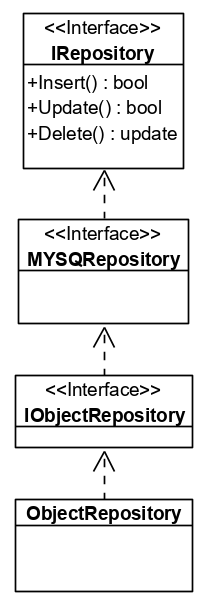
\includegraphics[width=0.2\textwidth]{figures/GenericRepositoryStructure.PNG}
    \caption{\textbf{PLACEHOLDER} repository diagram}
    \label{fig:RepositoryDiagram}
\end{figure}

The system specific structure of the implementation can be seen on \autoref{fig:RepositoryDiagram} this pattern is used to make it easier to change database system at a later date. \\
Any database implemented into the system needs to implement the different interfaces. As seen in \autoref{fig:RepositoryDiagram} all of the database related repositories depend on \textit{IRepository} this is done to ensure that the database interfaces implement \textbf{\textit{Insert()}}, \textbf{\textit{Update()}} and \textbf{\textit{Delete()}} as functions. By integrating these interfaces they satisfy the general needs for database implementations. \\
Depending on which repository is used (\textit{Asset},\textit{Log},\textit{Tag}, etc.) different functionalities needs to be implemented, this is done through the next layer of interfaces. The interfaces on the third layer defines the object specific functionalities, which the individual repository classes should implement. These classes handle the connections to the database, and handles the SQL scripts to the database, as well as constructing these scripts to fit to the specific model. \\
As some of the models have unique ways of being searched/added/edited in the database, individual interfaces were needed for these, to make sure the objects were saved and loaded correctly. \\
In the bottom of \autoref{fig:RepositoryDiagram} the object repository is defined, this class contains all the information and functions related to a specific model. This class contains the object specific implementation of all the functions defined in the chain of the interfaces. \\
If a new database structure where to be added at a alter date it would just have to define a dependency to the last of the "ObjectRepository", and will hereby be forced to implement the required functions, to make the database connection useful.
